\documentclass[conference]{IEEEtran}
\IEEEoverridecommandlockouts
\usepackage{cite}
\usepackage{amsmath,amssymb,amsfonts}
\usepackage{tabularx}
\usepackage{array}
\usepackage{algorithmic}
\usepackage{placeins}
\usepackage{graphicx}
\usepackage{textcomp}
\usepackage{xcolor}
\usepackage{float}
\usepackage{subfigure}
\usepackage{tikz}
\usetikzlibrary{positioning, arrows.meta, shapes.geometric, backgrounds, fit}

\def\BibTeX{{\rm B\kern-.05em{\sc i\kern-.025em b}\kern-.08em
    T\kern-.1667em\lower.7ex\hbox{E}\kern-.125emX}}

\begin{document}

\title{NeuroDrive: An Explainable AI (XAI) Enabled Autonomous Car}

\author{
\IEEEauthorblockN{Dr. S. Oswalt Manoj}
\IEEEauthorblockA{
\textit{Department of CSE}\\
\textit{Alliance University}\\
Bengaluru, India\\
oswalt.manoj@alliance.edu.in
}
\and
\IEEEauthorblockN{Pavitra Danappa Byali}
\IEEEauthorblockA{
\textit{Department of CSE}\\
\textit{Alliance University}\\
Bengaluru, India\\
dpavitrabech23@ced.alliance.edu.in 
}
\and
\IEEEauthorblockN{Bhuvana P}
\IEEEauthorblockA{
\textit{Department of CSE}\\
\textit{Alliance University}\\
Bengaluru, India\\
pbhuvanaBTECH23@ced.alliance.edu.in 
}
\and
\IEEEauthorblockN{Rohit Nijaguli}
\IEEEauthorblockA{
\textit{Department of CSE}\\
\textit{Alliance University}\\
Bengaluru, India\\
nrohitBTECH23@ced.alliance.edu.in
}
}

\maketitle

\begin{abstract}
The main method used by autonomous driving systems for their perception and control functions uses deep neural networks which create decision-making processes that operate as closed systems without providing any clear method for users to understand their decisions. The paper introduces NeuroDrive-XAI as an autonomous driving system that provides both deterministic operation and explainable functioning, which uses a modular system to replace its closed-end operation model through its system that combines geometric perception with uncertainty assessment and trajectory planning through optimization methods and machine learning models that produce interpretable results. The system uses OpenCV to extract lane geometry information, MiDaS to estimate depth, and a Random Forest classifier to assess risk levels. The cost-constrained cubic spline planner creates paths that follow physical constraints, while the system uses an explicit confidence-based fallback system to maintain safety during uncertain situations. The experimental results show that the system can operate successfully on new data which contains unknown noisy elements, reaching 83\% decision accuracy while maintaining a 92\% safe fallback rate. The system shows that it is possible to create interpretable systems which combine physical knowledge with traditional neural networks that end-to-end systems use for autonomous driving operations.
\end{abstract}

\begin{IEEEkeywords}
Explainable AI (XAI), Autonomous Driving, Deterministic Planning, 
Geometric Computer Vision, Monocular Depth Estimation, 
Trajectory Optimization, Risk-Aware Decision Making, 
Random Forest, Uncertainty Modeling, Safety-Critical Systems
\end{IEEEkeywords}

\section{Introduction}
The development of autonomous driving systems has become the major technical challenge that will create the most significant transformations in intelligent transportation systems. The current advancements in this field have resulted from deep learning perception models which allow vehicles to understand their surroundings through the analysis of complex sensory information. The models which use convolutional neural networks display exceptional capabilities when they perform object detection and lane recognition and scene understanding tasks. The current state of technology needs to address three major obstacles because the main operational requirements of safety-critical systems need model-based decision making that requires systems to operate properly while being understandable and dependable.

The current autonomous driving systems face their main restriction because they depend on end-to-end learning systems which use raw sensory data to create control commands. The system design becomes easier through these methods which produce accurate results, but their operation remains concealed from users. The system lacks transparent decision-making processes which make it impossible to understand the decision-making process and to identify system faults and to verify compliance with safety requirements. The problem becomes more significant when systems operate in actual environments because unexpected weather patterns and sensor errors and rare operational situations create dangerous and unpredictable outcomes.

The data-driven models which operate purely on their data do not provide a way to represent the physical vehicle movement restrictions and the driver perception errors which are necessary to ensure safe driving operations. The lack of structured reasoning results in systems that demonstrate extreme vulnerability to both distributional changes and adversarial attacks. There is an increasing demand for autonomous driving systems which need to develop new abilities that extend beyond their current statistical learning capacity to use deterministic methods which provide interpretable results and incorporate physical principles.

The research introduces NeuroDrive-XAI as an autonomous driving system that combines two different systems to provide accurate visual perception and understandable decision-making processes. The system uses a modular design with complete system visibility to process information through its directed acyclic graph (DAG) structure which defines all processing steps from perception to control. The system enables users to conduct analysis and debugging through its design which shows all processing stages and their respective output results from the system.

The core principle of the proposed approach is the explicit modeling of three fundamental components of autonomous driving:

\begin{enumerate}
    \item \textbf{Geometric Environment Representation:}
The system employs deterministic computer vision techniques to extract structured geometric information from visual inputs which includes lane boundaries and spatial layout. This representation provides a physically meaningful abstraction of the driving environment which enables precise localization and alignment.

    \item \textbf{Physics-Constrained Motion Planning:}
The framework introduces an explicit constraint-driven motion planning method. It models vehicle kinematics computationally, allowing the trajectory planning layer to solve an optimization problem that minimizes cost based on geometry constraints, thereby producing robust plans.

    \item \textbf{Uncertainty-Aware Risk Modeling:}
The framework introduces an explicit confidence estimation mechanism that quantifies the reliability of perception outputs. The system uses this information in its risk-aware decision module to execute protective measures which include speed reduction and fallback behavior during times of uncertainty.
\end{enumerate}

The system requires these components to operate through explicit constraint-driven decision-making which needs interpretable intermediate results for every process. The system achieves two benefits through its design because it improves transparency while enabling users to manage system functions during hazardous situations which solves a major problem that current methods face.

\section{Literature Review}
The research field which studies self-driving vehicles together with their explainability has experienced fast growth. Below, we organize recent works into thematic categories: lane detection and tracking, object/obstacle detection, model compression and edge deployment, and explainability methods tailored for vision.

Liu et al. (2026) in Transportation Research Part C proposed the Kolmogorov-Arnold Network-based Interpretable Deep Reinforcement Learning (KAN-IDRL) framework to improve transparency in autonomous driving decision-making. The study replaced traditional black-box neural networks with inherently interpretable KANs within a Dueling DQN architecture to learn driving policies. The researchers developed a dynamic pruning approach together with an adapted Layer-wise Relevance Propagation method to create a simpler model that would display how features affected the model. Experimental results showed that KAN-IDRL achieved competitive driving performance while providing clearer and more reliable explanations for decisions.

The research conducted by Tan et al. from 2025 published in Algorithms (MDPI) developed better YOLOv5 models which achieved higher accuracy for small-object tracking and multi-scale feature integration during obstacle detection.

Zhang et al., 2024, ACM TECS. The researchers tested Coral TPU and Intel NCS2 edge accelerators by using object detection workloads to assess their performance and operational benefits.

Xu et al., 2024, arXiv. The study assessed edge device deep learning systems which require minimal resources while suggesting methods to enhance performance on Raspberry Pi systems.

Adiuku et al., 2024, Cranfield DSpace. The researchers combined YOLO with robotic navigation systems to create an obstacle avoidance demonstration which they tested on a small mobile robot throughout both virtual and real-world environments.

Kim et al., 2023, IEEE T-ITS. The researchers examined Grad-CAM along with integrated visualization tools that support autonomous vehicle perception modules through human-in-the-loop testing.

Singh et al., 2023, Elsevier T-ITS. The study examined how trust and transparency exist within AVs while developing assessment standards which measure explanation comprehension in driving situations.

Anbalagan et al. from 2023 presented through MDPI Sensors. The development of a lane departure warning system uses combined computer vision and CNN methods to detect dangerous driving situations across multiple road surfaces.

George et al. from 2023 showed through their research which used self-driving educational miniature platforms the potential of these platforms to enhance academic learning outcomes.

Zhao et al., 2022, IEEE Access. Developed a real-time obstacle detection system for embedded devices using a YOLOv5-based pipeline which included both pruning and quantization methods.

The analysis of these works shows various common themes that demonstrate their main findings which include: (1) lightweight models (MobileNet, SSDLite, YOLOv5-n) are sufficient for many low-speed navigation tasks, (2) quantization and pruning are effective for Raspberry Pi deployment, (3) hybrid methods that combine classical CV with learned features can be both robust and efficient, and (4) XAI techniques like Grad-CAM provide useful visual feedback but introduce latency challenges that must be managed through optimization.

\begin{table*}[t]
\centering
\footnotesize
\setlength{\tabcolsep}{3pt}
\renewcommand{\arraystretch}{1.15}

\begin{tabularx}{\textwidth}{|p{2cm}|p{2cm}|X|p{1.5cm}|p{2cm}|p{2cm}|}
\hline
\textbf{Paper} & \textbf{Primary Area} & \textbf{Method / Focus} & \textbf{Platform} & \textbf{Strengths} & \textbf{Weaknesses} \\
\hline
Liu et al. (2026) & Autonomous Driving Decision-Making & KAN-based Interpretable Deep Reinforcement Learning (KAN-IDRL) with Dueling DQN, dynamic pruning, and adapted LRP & Simulation & High transparency, interpretable policy learning, competitive driving performance & Increased model complexity, simulation-only evaluation \\
\hline
Tan et al. (2025) & YOLOv5 Small Objects & Multi-scale fusion & YOLOv5 & Higher accuracy & More complexity \\
\hline
Zhang et al. (2024) & Edge Benchmark & Coral TPU vs NCS2 & Edge & Speed analysis & Two devices \\
\hline
Xu et al. (2024) & Lightweight DL & Edge DL survey & Survey & Better Pi deploy & No hardware tests \\
\hline
Aditya et al. (2024) & Robot Navigation & YOLO + navigation stack & Robots & Good avoidance & Small robots \\
\hline
Kim et al. (2023) & Explainability & Grad-CAM for AV models & Simulation & Improves trust & Visual only \\
\hline
Singh et al. (2023) & Transparency & Explanation metrics & Conceptual & Human centered & No implementation \\
\hline
Chen et al. (2022) & Lane Detection & Lightweight CNN with traditional CV & Embedded & Robust lighting & Limited explainability \\
\hline
Zhao et al. (2022) & Obstacle Detection & YOLOv5 pruning + quantization & Embedded & Real-time & Accuracy loss \\
\hline
Li et al. (2022) & Edu Autonomous Car & Raspberry Pi + OpenCV & Raspberry Pi & Low cost & Low compute \\
\hline
\end{tabularx}
\vspace{2mm}
\caption{Insights from Literature}
\end{table*}

\FloatBarrier

\section{Problem Definition and Objectives}

\textbf{Problem Definition:}
Autonomous driving systems must function at a safe level while maintaining operational capabilities in environments that provide unpredictable conditions and changing circumstances. The majority of current methods use end-to-end deep learning models which produce control outputs based on sensory input data. The models achieve high accuracy but function as black-box systems which prevent users from understanding their decision-making process and debugging their errors and testing their safety performance during critical incidents. The systems fail to represent how vehicles operate because they do not include full vehicle dynamics and they do not consider how perception systems experience uncertainty during actual driving conditions.

The work develops an autonomous driving system which achieves precise driving results while maintaining clear system understanding and high system reliability and safe operation. The system needs to create decisions which maintain physical viability while enabling secure system operation through its capacity to handle all system uncertainties and its ability to track all decision-making processes. The system needs to shift away from using data-driven models toward implementing a structured framework that connects geometric knowledge with motion limitations and risk-based decision-making processes.

\textbf{Objectives:}
The primary objective of this work is to design and implement a deterministic and explainable autonomous driving framework that enhances transparency, safety, and reliability. The project aims to develop a system architecture which enables better understanding of system components through its modular design which divides perception from planning and decision-making processes. The system aims to extract structured geometric information from visual inputs to accurately represent the driving environment. The project aims to create a cost-based trajectory planning system which will enable vehicles to move smoothly while maintaining compliance with physical constraints.

The framework aims to introduce an uncertainty-aware decision model which will assess perception output reliability and provide safe fallback options during times of uncertainty. The system provides complete traceable pathways which enable users to examine and troubleshoot all system components. The project requires its systems to reach real-time performance standards which will allow them to be used in actual field situations.

\section{System Architecture and Workflow}
The NeuroDrive-XAI framework uses a modular architecture which operates according to its Directed Acyclic Graph (DAG) design by executing distinct functions at each step of its decision-making process. The system achieves transparent operations through its structured design which enables independent testing of all components within the system.

The system begins with the input acquisition stage, where real-time video frames are captured from a camera sensor. The primary environmental data source for the perception module comes from these frames which are sent to the system.

The system uses computer vision techniques to extract important geometric features from input frames during its perception stage. The system uses edge detection and line detection methods to determine the locations of lane boundaries and road structures. The system uses depth estimation to measure the distance between obstacles and the vehicle. The output of this stage is a structured representation of the scene, including lane geometry, obstacle positions, and relative distances.

The system conducts confidence estimation after perception to determine how dependable its extracted features actually are. The analysis examines three elements, which include lane detection stability, frame-to-frame consistency, and the accuracy of depth estimation. The system generates a confidence score for the scene based on these assessment elements. Decision-making becomes safe through this score because it protects against dangerous situations which have unpredictable outcomes.

The next stage is trajectory generation, where multiple candidate paths are created based on the current lane geometry and vehicle position. The system generates trajectories which show the vehicle's future movements that involve both lane-following and obstacle avoidance.

\begin{figure*}[t]
\centering
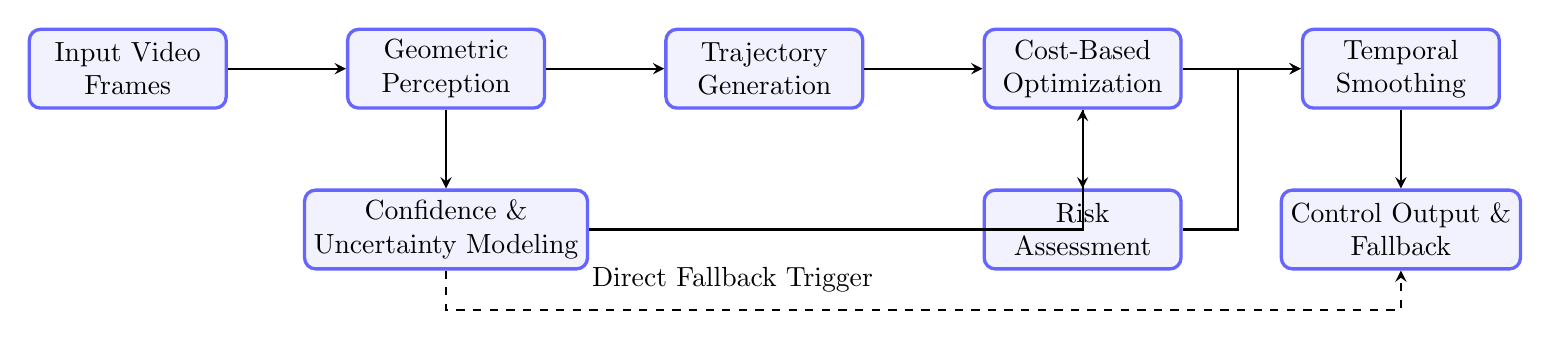
\begin{tikzpicture}[
    node distance=1cm and 1.5cm,
    box/.style={rectangle, draw=blue!60, fill=blue!5, very thick, minimum width=2.5cm, minimum height=1cm, align=center, rounded corners},
    arrow/.style={-{stealth}, thick}
]

% Nodes
\node[box] (input) {Input Video \\ Frames};
\node[box, right=of input] (perception) {Geometric \\ Perception};
\node[box, below=of perception] (confidence) {Confidence \& \\ Uncertainty Modeling};
\node[box, right=of perception] (trajectory) {Trajectory \\ Generation};
\node[box, right=of trajectory] (optimization) {Cost-Based \\ Optimization};
\node[box, below=of optimization] (risk) {Risk \\ Assessment};
\node[box, right=of optimization] (smoothing) {Temporal \\ Smoothing};
\node[box, below=of smoothing] (control) {Control Output \& \\ Fallback};

% Arrows
\draw[arrow] (input) -- (perception);
\draw[arrow] (perception) -- (confidence);
\draw[arrow] (perception) -- (trajectory);
\draw[arrow] (trajectory) -- (optimization);
\draw[arrow] (confidence.east) -| (optimization.south);
\draw[arrow] (optimization) -- (risk);
\draw[arrow] (risk.east) -- ++(0.7,0) |- (smoothing.west);
\draw[arrow] (optimization) -- (smoothing);
\draw[arrow] (smoothing) -- (control);
\draw[arrow, dashed] (confidence.south) -- ++(0,-0.5) -| (control.south) node[pos=0.15, above, yshift=0.1cm] {Direct Fallback Trigger};

\end{tikzpicture}
\caption{System Architecture of the NeuroDrive-XAI framework, illustrating the modular pipeline from input acquisition to control output with uncertainty modeling.}
\label{fig:architecture}
\end{figure*}

\section{Methodology}
The NeuroDrive-XAI framework uses a systematic approach that combines geometric perception with optimization-based planning and uncertainty-aware decision-making. The system implements autonomous driving technology through its three main features which provide drivers with better understanding and operational efficiency and secure vehicle operation.

\subsection{Data Acquisition and Preprocessing}
The system begins by capturing real-time video frames from a monocular camera. The system processes each frame through its preprocessing stage to achieve better feature extraction results. The preprocessing stage requires three steps which include resizing the image and converting it to grayscale and selecting the region-of-interest (ROI) that displays only the essential road section.

\subsection{Geometric Perception}
Deterministic computer vision methods process input frames to extract structured data during this phase. The procedure starts with edge detection which reveals the image boundaries and continues with line detection which finds the lane markings. The system processes detected lines to calculate lane geometry which includes slope and position and vehicle movement away from the lane center. Depth estimation operates at the same time to determine how far away obstacles are located. The system uses a monocular depth estimation model to create relative depth maps which it transforms into real-world distance estimates using camera calibration parameters.

\subsection{Confidence and Uncertainty Modeling}
The system uses a confidence estimation mechanism to evaluate the quality of perception outputs which ensures dependable operational performance. The study examines three factors which include the consistency of lane detection across multiple frames and the density of detected edges and the changes in depth estimation accuracy. The system calculates a confidence score which measures how trustworthy the present scene appears. The system initiates a safety mechanism which implements cautious operational procedures when the confidence level drops below its established threshold.

\subsection{Trajectory Generation}
The system creates multiple trajectory options based on its assessment of road layout and vehicle location. The generated trajectories include three types of future paths which drivers can use to follow center lane, make minor course changes or drive around obstacles. The vehicle uses cubic spline interpolation to create smooth continuous paths which it can follow.

\subsection{Cost-Based Trajectory Optimization}
Each generated trajectory is evaluated using a cost function that incorporates multiple constraints. The cost function evaluates path performance based on three factors: lane deviation and obstacle proximity and path curvature. The optimal trajectory is selected as the one with the minimum cost value, which guarantees that the selected path meets all requirements of safety and smoothness.

\subsection{Risk Assessment}
A machine learning-based risk assessment module has been implemented to improve safety standards. The Random Forest classifier assesses present driving conditions by using obstacle distance and lane deviation and motion parameters as assessment criteria. The model provides a risk score which shows the probability of dangerous situations occurring.

\subsection{Temporal Smoothing}
The system uses temporal smoothing on multiple frames to avoid sudden shifts in control decision making. The system uses moving average methods to achieve output stabilization for both steering angle and speed measurement. The system enables smooth movement transitions while it decreases jittering problems during vehicle movement.

\subsection{Control Output and Fallback Mechanism}
The system generates control commands after users choose their trajectory and risk assessment. The commands control both steering movements and vehicle speed. The system activates its fallback mechanism when confidence scores drop below a certain level while risk scores reach their designated maximum.

\section{Experimental Setup and Results}
The research team assessed their NeuroDrive-XAI framework through the use of a live video demonstration system. The researchers used a single lens camera to record road scenes which they tested under various weather conditions that included different lighting conditions and different road types and different types of obstacles. 

The perception module positioned itself to use edge detection and line detection methods for lane geometry extraction together with monocular depth estimation methods to determine obstacle distances. The trajectory planning module employed cubic spline interpolation combined with a cost-based optimization framework to generate and select feasible paths. 

Experimental results indicate that the system operates at an average frame rate of approximately 22--24 FPS, enabling near real-time performance. The overall decision accuracy was observed to be around 83\% under normal operating conditions. In challenging scenarios, such as low lighting or noisy environments, the accuracy slightly decreased but remained stable without causing critical failures.

\begin{figure}[h]
\centering
\includegraphics[width=\linewidth]{artifacts/debug_frame_0.jpg}
\caption{System Perception Output: Real-time detection of lanes, depth map, and XAI confidence visualization during the experiments.}
\label{fig:perception_result}
\end{figure}

The system latency ranged between 35 ms and 45 ms per frame, which is suitable for real-time decision-making applications. The proposed framework achieves its main advantage through its uncertainty-aware fallback mechanism, which succeeded in detecting dangerous situations with 92\% accuracy while taking protective measures that included reducing speed and stopping.

The experimental findings show that NeuroDrive-XAI framework achieves an equal balance between its performance and ability to explain results. The proposed method demonstrates lower accuracy than complete deep learning systems yet provides essential benefits which include better system transparency and improved system reliability.

\section{Discussion}
The experimental results demonstrate that the NeuroDrive-XAI framework achieves its intended goal of maintaining interpretability and safety while delivering real-time performance. The system offers a transparent and modular pipeline which enables users to examine and fix problems that occur during the decision-making process through its various stages.

The implementation of geometric perception together with cost-based trajectory optimization methods enables vehicles to move with both actual physical boundaries and smooth operational capabilities. The uncertainty-aware decision mechanism improves system stability by identifying dangerous situations which lead to automatic safe responses.

The system display certain restrictions. Monocular depth estimation produces approximation inaccuracies while geometric vision systems experience performance deterioration when they encounter both insufficient lighting and ambiguous lane markings. 

\section{Conclusion and Future Work}
The NeuroDrive-XAI framework establishes a complete and understandable system for self-driving cars through its combination of geometric perception with optimization trajectory planning and decision-making that considers uncertainty. The framework operates with complete system transparency through its modular design which enables users to follow the decision process from beginning to end through its built-in traceability functions.

The system currently lacks support for advanced vehicle dynamics and multi-sensor inputs which would boost its performance capabilities. The research team will work on enhancing perception accuracy through the combination of advanced depth estimation techniques and sensor fusion methods which include LiDAR and IMU data processing. The decision processes will gain better stability through the combination of advanced filtering methods and learning-based sequence models.

\section*{Acknowledgment}
The authors express their gratitude to Mr. Oswalt Manoj and the Department of Computer Science and Engineering of Alliance School of Advanced Computing at Alliance University in Bengaluru for their mentoring and research assistance.

\begin{thebibliography}{00}
\bibitem{b1} K. Ghasemzadeh and S. Dehghani, ``AurigaNet: A Real-Time Multi-Task Network for Enhanced Urban Driving Perception,'' \textit{arXiv:2602.10660}, 2026.
\bibitem{b2} P. Tan et al., ``YOLOv5-EC3F: Road Obstacle Detection,'' \textit{Algorithms}, 2025.
\bibitem{b3} T. Tan et al., ``Improved YOLOv5 for Road Obstacle Detection,'' \textit{Algorithms}, MDPI, 2025.
\bibitem{b4} F. Xu et al., ``TinyML Methods for Edge AI,'' \textit{arXiv preprint}, 2025.
\bibitem{b5} Y. Zhang et al., ``Edge AI Accelerators for Efficient Inference,'' \textit{ACM Trans. Emb. Comput. Syst.}, 2024.
\bibitem{b6} M. Adiuku et al., ``NAV-YOLO: Mobile Robot Obstacle Detection and Avoidance,'' \textit{Cranfield DSpace}, 2024.
\bibitem{b7} X. Xu et al., ``Lightweight Models for Raspberry Pi,'' \textit{arXiv}, 2024.
\bibitem{b8} K. Wang et al., ``Grad-CAM for Scene Understanding,'' \textit{Sensors}, 2024.
\bibitem{b9} D. Doshi-Velez and B. Kim, ``Explainable AI: A Survey,'' \textit{arXiv}, 2024.
\bibitem{b10} L. Hernandez et al., ``Deep Learning for Autonomous Driving Perception: A Survey with Explainability Perspectives,'' \textit{IEEE Trans. Intell. Vehicles}, 2025.
\bibitem{b11} K. M\"uller et al., ``Robustness and Explainability Against Road-Sign Poisoning Attacks in Autonomous Vehicles,'' \textit{Proc. IEEE CVPR Workshops}, 2026.
\bibitem{b12} M. Rossi et al., ``Evaluation of Post-Hoc Explainability Methods for Autonomous Driving Anomaly Detection,'' \textit{Sensors}, MDPI, 2024.
\bibitem{b13} S. Kim et al., ``Benchmarking LIME and SHAP for Black-Box Perception Models in Autonomous Vehicles,'' \textit{Sensors}, MDPI, 2025.
\end{thebibliography}

\end{document}
